%version of 10-16-19
\chapter{$\oplus$ Hamiltonianicity in Weighted Graphs: the TSP}
\label{sec:TSP}
\index{Traveling Salesman Problem}
\index{TSP: the Traveling Salesman Problem}

This chapter deals with an algorithmic problem which exercises several important graph-theoretic concepts and constructs.  It affords the reader the chance to observe material from Chapters~\ref{ch:Graphs1} and~\ref{ch:Graphs2} ``in action".

\medskip

In Section~\ref{sec:Hamiltonian-unweighted}, we suggested how daunting it is computationally to determine whether an unweighted graph admits a Hamiltonian cycle.  There is an important, practically significant, analogue of this problem for edge-weighted graphs, which has traditionally been known as the {\it Traveling Salesman Problem}; we shall use instead the modern abbreviation {\it TSP}.  The TSP is a classical problem in the field of Operations Research, whose familiar name arises from the following story.

\index{Traveling Salesman Problem!origin of the name}

\smallskip

We consider a saleswoman who wants to make a call on all of her $n$ clients, who live in the $n$ cities, $C_1, C_2, \ldots, C_n$.  In order to minimize the cost of her tour, she studies the
$\displaystyle {n \choose 2}$ real numbers $\{c_{i,j} \ | \ 1 \leq i,j \leq n\}$, where each $c_{i,j}$ is the {\it cost} of traveling from city $C_i$ to city $C_j$.  Since our prime concern is in the underlying mathematics rather than in the governing algorithmics, we shall simplify the setting of the TSP to situations wherein intercity costs are {\em commutative}, so that each  $c_{i,j}$ is the {\it cost} of traveling {\em between} city $C_i$ and city $C_j$ {\em in either direction}.

\bigskip

\noindent \fbox{
\begin{minipage}{0.95\textwidth}
We are purposely vague about the meaning of the word ``cost'' in this problem.  The costs represented by the unknowns $c_{i,j}$ could be intercity driving distances or inter-region travel times or international airfares.  Instances of the TSP can be formulated with {\em any} notion of cost that can be represented by positive real numbers.

\smallskip

\index{triangle inequality} \index{Euclidean distance measure} \index{Euclid}
The importance of being vague is that {\em costs are not assumed to obey any of the laws that one commonly associates with the distances we encounter in our daily lives}.  The
{\it triangle inequality} is a prime example of such a law.  Essentially, this law insists that the
distance between two cities is never decreased by placing an intermediate stopover city between them: It is a discretization of the geometric postulate, {\em A straight line is the shortest distance between two points.}  Cost measures that obey the triangle inequality are termed {\it Euclidean} because the distances studied in Euclidean plane geometry are assumed to obey this law.

\smallskip

Some people like to think of general intercity costs as airfares---which clearly obey no immutable laws.
\end{minipage}
}
\bigskip

The saleswoman's objective is to schedule the order of visiting her clients' $n$ cities in the most economical way.  Formally, the challenge of the TSP is to discover a {\em minimum-cost tour} of all $n$ cities.  Such a tour would be a cycle of the form

\hspace*{.35in} $C_{i_1}$--$C_{i_2}$-- $\cdots$ --$C_{i_n}$--$C_{i_1}$

\noindent such that:
\begin{itemize}
\item
all $n$ cities appear in the tour precisely once;
\item
no tour has cost smaller than the cost
\[ c_{i_1,i_2} \ + \ c_{i_2, i_3} \ + \cdots + \ c_{i_{n-1}, i_n} \ + \ c_{i_n, i_1}
\]
of the indicated tour.
\end{itemize}
The main connection of the TSP to our study of paths and cycles in graphs is twofold.
\begin{enumerate}
\item
The TSP can be represented as a weighted analogue of the problem of detecting Hamiltonian cycles (as studied in Section~\ref{sec:Hamiltonian-cycle}).  Within this representation: the TSP's $n$ cities are depicted as an instance of the complete graph $\k_n$; its intercity costs are real-number weights on the edges of $\k_n$.\footnote{When intercity distances are not commutative, we must deal with the {\em directed} version of $\k_n$.}  We describe this representation via the following informal, but precise, encoding of an arbitrary $n$-vertex graph $\g$ as an instance of the TSP.
  \begin{itemize}
  \item
Each vertex of $\g$ becomes a city that must be visited.  To emphasize this representation, we denote $\g$'s vertex-set as $\{C_1, C_2, \ldots, C_n\}$.
  \item
We posit the following intercity costs.  For each pair of cities $C_i$ and $C_j$:
\[ c_{i,j} \ = \ \left\{
\begin{array}{ccl}
1 & & \mbox{if there is an edge between $C_i$ and $C_j$ in $\g$} \\
\infty & & \mbox{if there is no edge between $C_i$ and $C_j$ in $\g$} \\
       & & \mbox{\small\sf (if the idea of ``infinite'' costs bothers you, then} \\
       & & \mbox{\small\sf make this some ``ridiculously large" number)}
\end{array}
\right.
\]
\end{itemize}

\item
The TSP is computationally ``no easier'' than the Hamiltonianicity-detection problem, in a very strong sense.  By definition, the target of the TSP is a tour of minimum {\em cumulative cost}, as measured by the sum of the costs of the edges traversed in the tour.  But, of course, {\em every} tour has some cost, according to this measure.  The computational difficulty of the TSP is suggested by the following result, which we state without proof.
\end{enumerate}

\begin{prop}[\cite{GareyJ79}]
\label{thm:Approx-TSP-NPC}
For any fixed positive constant $\kappa$, the problem of finding a tour for an instance of the TSP that is within a factor of $\kappa$ of minimal is an {\sf NP}-complete problem.
\end{prop}

\index{Euclidean TSP problem} 
\index{Traveling Salesman Problem!approximately optimal solution}
\index{TSP: the Traveling Salesman Problem!approximately optimal solution} 

It should be no surprise to the reader that the TSP is a computationally complex problem, in the light of our just-described encoding of the TSP as a form of the Hamiltonianicity-detection problem.  What is surprising, though, is that if we restrict attention to {\em Euclidean} instances of the TSP---i.e., instances whose ``costs'' measure Euclidean distances (say, e.g., driving distances), then there exists a rather efficient algorithm which solves such instances of the TSP {\em approximately} optimally, in the sense of Proposition~\ref{thm:Approx-TSP-NPC}.  %Specifically, for each {\em Euclidean} instance $\i$ of the TSP that has an {\em optimal/cost-minimal} of cost $c[\i]$, algorithm $\a$ discovers a tour whose cost is no larger than $\kappa \cdot c[\i]$.
This algorithm is typically known by the name of its inventor, Nicos Christofides.
\index{Christofides, Nicos}

\begin{prop}[\cite{Christofides76}]
\label{thm:Christofides}
There exists an algorithm for the Euclidean TSP that produces tours whose costs are no greater than $1.5$ times the cost of an optimal tour.
\end{prop}

The proof of Proposition~\ref{thm:Christofides} develops the rather sophisticated claimed approximation algorithm.  We refer the reader to an algorithms text such as \cite{CLRS} for the details.  We choose instead to sketch a much simpler algorithm, which achieves an approximation factor of $2$, while exposing most of the graph-theoretic ideas in the full proof.   

The factor-of-$2$ approximation algorithm begins with the cost matrix

\ignore{***************. **HERE**
The following table, and Fig.~\ref{fig:perfectMatchingInitial}, depict
an instance of the Euclidian TSP with $n=7$ cities.
\[
\begin{array}{|c||c|c|c|c|c|c|c|}
\mbox{\bf City} & \multicolumn{6}{c}{\mbox{\bf Inter-City Costs}} \\
\hline
C_1 & 0 & c_{1,2} & c_{1,3} & c_{1,4} & c_{1,5} & c_{1,6} & c_{1,7} \\
\hline
C_2 & c_{2,1} & 0 & c_{2,3} & c_{2,4} & c_{2,5} & c_{2,6} & c_{2,7} \\
\hline
C_3 & c_{3,1} & c_{3,2} & 0 & c_{3,4} & c_{3,5} & c_{3,6} & c_{3,7} \\
\hline
C_4 & c_{4,1} & c_{4,2} & c_{4,3} & 0 & c_{4,5} & c_{4,6} & c_{4,7} \\
\hline
C_5 & c_{5,1} & c_{5,2} & c_{5,3} & c_{5,4} & 0 & c_{5,6} & c_{5,7} \\
\hline
C_6 & c_{6,1} & c_{6,2} & c_{6,3} & c_{6,4} & c_{6,5} & 0 & c_{6,7} \\
\hline
C_7 & c_{7,1} & c_{7,2} & c_{7,3} & c_{7,4} & c_{7,5} & c_{7,6} & 0 \\
\hline
\end{array}
\]
\begin{figure}[hbt]
\begin{center}
       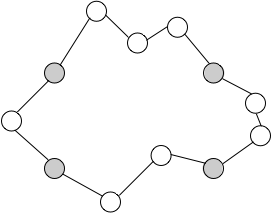
\includegraphics[scale=0.7]{FiguresGraph/perfectmatching1}
       \caption{An optimal Hamiltonian cycle $H^*$.}
              \label{fig:perfectMatchingInitial}
\end{center}
\end{figure}
******************}

\ignore{*********
It corresponds to determine a minimal Hamiltonian cycle in a weighted
complete graphs $K_n$.  Obviously, $K_n$ is Hamiltonian (it exists
$n!$ such Hamiltonian paths), thus, the question here is to determine
the minimum one.

  Of course, she must go in every city and her objective is to
minimize the total distance done in the tour.  The only information
she has is the list of the cities and a map with all inter-cities
distances.  We assume a \textit{Euclidian distance} (for instance the
weights correspond to number of kilometers between two cities).  This
property means that the straight line is always the minimum distance,
or in other words that the distance between two vertices/cities is
larger if the path is going through any other vertex.
%More formally, the input of the problem is a weighted matrix with an infinite weight on the diagonal.
\bigskip
*****************}



Proving this result is the domain of an algorithms text---see, e.g., \cite{CLRS}.  We remark here only that the algorithm of Christofides combines a number of classical computational problems that admit efficient solutions: minimum-weight spanning trees, preorder walks within trees, and
minimum-weight perfect matchings.

\bigskip

We construct an efficient solution for the Euclidean TSP, which is
known as {\it the Christofides algorithm}, \index{Christofides algorithm} 
after its inventor, Nicos Christofides.
\index{Christofides, Nicos}
\cite{Christofides76}

The following table, and Fig.~\ref{fig:perfectMatchingInitial}, depict
an instance of the Euclidian TSP with $n=7$ cities.
\[
\begin{array}{|c||c|c|c|c|c|c|c|}
\mbox{\bf City} & \multicolumn{6}{c}{\mbox{\bf Inter-City Costs}} \\
\hline
C_1 & 0 & c_{1,2} & c_{1,3} & c_{1,4} & c_{1,5} & c_{1,6} & c_{1,7} \\
\hline
C_2 & c_{2,1} & 0 & c_{2,3} & c_{2,4} & c_{2,5} & c_{2,6} & c_{2,7} \\
\hline
C_3 & c_{3,1} & c_{3,2} & 0 & c_{3,4} & c_{3,5} & c_{3,6} & c_{3,7} \\
\hline
C_4 & c_{4,1} & c_{4,2} & c_{4,3} & 0 & c_{4,5} & c_{4,6} & c_{4,7} \\
\hline
C_5 & c_{5,1} & c_{5,2} & c_{5,3} & c_{5,4} & 0 & c_{5,6} & c_{5,7} \\
\hline
C_6 & c_{6,1} & c_{6,2} & c_{6,3} & c_{6,4} & c_{6,5} & 0 & c_{6,7} \\
\hline
C_7 & c_{7,1} & c_{7,2} & c_{7,3} & c_{7,4} & c_{7,5} & c_{7,6} & 0 \\
\hline
\end{array}
\]


\begin{figure}[hbt]
\begin{center}
       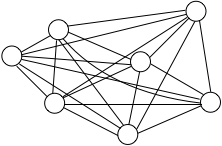
\includegraphics[scale=0.8]{FiguresGraph/christofides1}
\caption{An instance of the Euclidean TSP with $7$ cities, $C_1$,
  $C_2$, $C_3$, $C_4$, $C_5$, $C_6$, $C_7$, and intercity costs
  $\{c_{i,j} \ | \ 1 \leq i,j \leq 7\}$.}
              \label{fig:christofidesInitial}
\end{center}
\end{figure}


Let us construct a good solution (not \textit{too far} from the optimal) in polynomial time. 
Let us denote by $\omega_G$ the weight of graph G (i.e. the sum of the weights on its edges). 
The Christofides algorithm proceeds in three steps. 
\bigskip

\textbf{Step 1.} Determine a minimal weight spanning tree $T^*$. 
%A spanning tree of G is a tree (connected graph with no cycle) with the same set of vertices as G. 
As we recalled in the preliminaries, a minimal weight spanning tree can be determined in polynomial time. 
\bigskip

$\omega_{T^*}$ is a lower bound of the value of the optimal tour $\omega_{H^*}$. 
Indeed, $H^*$ is a cycle, then, removing any edge in $H^*$ leads to a chain, which is a particular spanning tree.
As $T^*$ is the minimal spanning tree, we have:
$\omega_{T^*} \leq \omega_{H^*}$.

\begin{figure}[hbt]
\begin{center}
       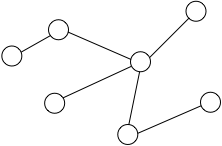
\includegraphics[scale=0.6]{FiguresGraph/christofides2}
       \caption{Construction of an optimal spanning Tree $T^*$.}
              \label{fig:christofidesSpanningTree}
\end{center}
\end{figure}


\textbf{Step 2.} Consider now the set $V_{odd}$ of the vertices of $T^*$ whose degrees are odd. 

We proved in the preliminary properties that the cardinality of $V_{odd}$ is even. 

Let us construct the perfect matching $C^*$ of minimum weight between the vertices in $V_{odd}$. 
Fig.~\ref{fig:AllPerfectMatchings} shows all possible perfect matchings on the previous example, the optimal one (with minimal weight) is represented in bold. 

Fig.~\ref{fig:christofidesPerfectMatching} illustrates the graph obtained by considering the edges of both $T^*$ and $C^*$. 
\begin{figure}[hbt]
\begin{center}
       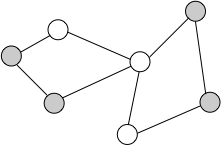
\includegraphics[scale=0.6]{FiguresGraph/christofides3}
       \caption{Adding the optimal perfect matching $C^*$ to the minimal spanning tree $T^*$.}
              \label{fig:christofidesPerfectMatching}
\end{center}
\end{figure}

Let us now determine a lower bound of the optimal tour $H^*$ (represented in Fig.~\ref{fig:perfectMatchingInitial}).

$2 \omega_{C^*}$ is a lower bound of the value of the optimal tour ($\omega_{C^*} \leq \frac{1}{2} \omega_{H^*}$). 
Indeed, consider first the perfect matching $C^*$.
As its vertices belong to $H^*$, $\omega_{C*}$ is lower than the piece of Hamiltonian tour contained between these vertices
because of the euclidian property (see Fig.~\ref{fig:perfectMatchingC*}).
Similarly for the \textit{complementary} perfect matching $C$ (Fig.~\ref{fig:perfectMatchingC}).  
Thus, the weight of the cycle formed by the concatenation of both perfect matchings 
is lower than the Hamiltonian tour $\omega_{C^* \bigcup C} \leq \omega_{H^*}$.
Moreover, as $C^*$ is the minimum perfect matching, we have $\omega_{C^*} \leq \omega_{C}$, 
this concludes the proof.


\begin{figure}[hbt]
\begin{center}
       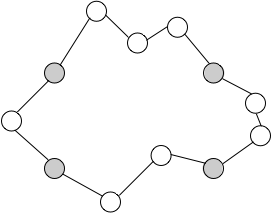
\includegraphics[scale=0.7]{FiguresGraph/perfectmatching1}
       \caption{An optimal Hamiltonian cycle $H^*$.}
              \label{fig:perfectMatchingInitial}
\end{center}
\end{figure}

\begin{figure}[hbt]
\begin{center}
       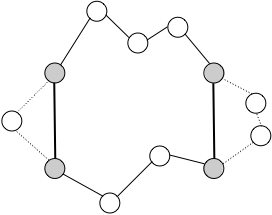
\includegraphics[scale=0.7]{FiguresGraph/perfectmatching2}
       \caption{Perfect matching $C^*$ between the vertices of odd degrees.}
              \label{fig:perfectMatchingC*}
\end{center}
\end{figure}

\begin{figure}[hbt]
\begin{center}
       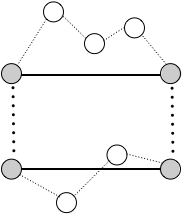
\includegraphics[scale=0.7]{FiguresGraph/perfectmatching3}
       \caption{Cycle $C^* \bigcup C$ (in dashed and bold).}
              \label{fig:perfectMatchingC}
\end{center}
\end{figure}

\bigskip

\textbf{Step 3.} 
All the vertices of $T^* \cup C^*$ have an even degree since we added an edge of $C^*$ to every odd degree vertices of $T^*$. 
We are now going to transform this graph by replacing iteratively the high degree vertices by shortcuts, 
which decreases the degree until reaching $2$. 

While it exists a vertex of degree greater than 4, we remove two of these consecutive edges and replace them 
by the opposite edge of this triangle 
without disconnecting the graph. 
There are $2k$ ways to remove $2$ edges and replace them by the triangle edge. 
Some of them disconnect the graph and thus, must be avoided. 
Fig.~\ref{fig:christofidesFinalStep1} shows such a transformation on the previous example, 
Fig.~\ref{fig:christofidesFinalStep2} shows a valid transformation.

\begin{figure}[hbt]
\begin{center}
       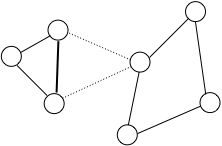
\includegraphics[scale=0.6]{FiguresGraph/christofides4}
       \caption{Reduction of the degree in $T^* \bigcup C^*$, disconnected solution.}
              \label{fig:christofidesFinalStep1}
\end{center}
\end{figure}

\begin{figure}[hbt]
\begin{center}
       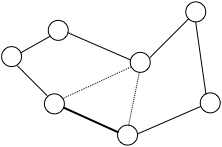
\includegraphics[scale=0.6]{FiguresGraph/christofides5}
       \caption{Reduction of the degree in $T^* \bigcup C^*$, connected solution.}
       \label{fig:christofidesFinalStep2}
\end{center}
\end{figure}

This process leads to a feasible tour. 
Such transformations do not increase the total weight.

Finally, 
as $\omega_{T^*} \leq \omega_{H^*}$ and $\omega_{C^*} \leq 1/2 \omega_{H^*}$,
we deduce that the value of such a tour is lower than $3/2 \omega_{H^*}$.
